% !TeX spellcheck = en_US
\documentclass[french]{yLectureNote}

\title{Optique ondulatoire}
\subtitle{Physique}
\author{Paulhenry Saux}
\date{\today}
\yLanguage{Français}

\professor{F.Pettinari}
\usepackage{graphicx}%----pour mettre des images
\usepackage[utf8]{inputenc}%---encodage
\usepackage{geometry}%---pour modifier les tailles et mettre a4paper
%\usepackage{awesomebox}%---pour les boites d'exercices, de pbq et de croquis ---d\'esactiv\'e pour les TP de PC
\usepackage{tikz}%---pour deiffner + d\'ependance de chemfig
% \usepackage{tabularx}%---pour dimensionner automatiquement les tableaux avec variable X
\usepackage{awesomebox}%---Pour les boites info, danger et autres
\usepackage{menukeys}%---Pour deiffner les touches de Calculatrice
\usepackage{fancyhdr}%---pour les en-t\^ete personnalis\'ees
\usepackage{blindtext}%---pour les liens
\usepackage{hyperref}%---pour les liens (\`a mettre en dernier)
\usepackage{caption}%---pour la francisation de la l\'egende table vers Tableau
\usepackage{pifont}
\usepackage{array}%---pour les tableaux
\usepackage{lipsum}
\usepackage{yFlatTable}
\usepackage{multicol}
\newcommand{\Lim}[1]{\lim\limits_{\substack{#1}}\:}
\renewcommand{\vec}{\overrightarrow}
\newcommand{\N}[0]{\mathbb{N}}
\newcommand{\dd}{\mathrm{d}}
\newcommand{\norm}[1]{||\vec{#1}||}
\newcommand{\fo}{\psi(\vec{r},t)}
\newcommand{\foe}{\psi(\vec{r},t)\*}
\newcommand{\HH}{\hat{H}}
\newcommand{\hb}{\hbar}
\newcommand{\lap}{\nabla^2}
\newcommand{\lapcc}{\frac{\partial^2 }{\partial x^2}+\frac{\partial^2 }{\partial y^2}+\frac{\partial^2 }{\partial z^2}}
\newcommand{\mpsi}{\(\psi\)}
\newcommand{\und}{\underline}
\newcommand{\dph}{\Delta\varphi}
\newcommand{\sinc}{\mathrm{sinc}}
\begin{document}
%TODO réviser optique géométrique
\setcounter{chapter}{2}
\chapter{Interférences d'ondes lumineuses}
\section{Introduction}
\begin{theorem}[Diffraction]
La diffraction d'une onde correspond à son étalement au cours de la propagation. C'est équivalent à un écart à la propagation rectiligne de la lumière.
\end{theorem}
Un faisceau laser collimaté de diamètre 1mm aura un diamètre de l'ordre du cm\marginCritical{Le phénomène se manifeste pour une onde dont la largeur est suffisamment petite}. On obtient à une certaine distance un faisceau conique au lieu d'un faisceau cylindrique.
\section{Principe de Huygens-Fresnel}
\subsection{Principe}
\warningInfo{Hypothèse}{L'onde est monochromatique de pulsation \(\omega\) avec \(k = n\frac{\omega}{c}\) et \(PM >> \lambda_0\)}
\begin{theorem}[Principe de Huygens]
 \[\und{\psi(M)} = \iint_{(P\in S)}k\und{\psi(P)} \frac{e^{ikPM}}{PM}\dd S \] avec K le facteur d'inclinaison
\end{theorem}
Cela signifie que si l'on connaît son profil sur une surface fermée, je peux calculer son expression partout.
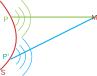
\includegraphics[scale=0.5]{huygens}
\checkInfo{Simplification}{On utilisera souvent une surface S plane comme un plan principal de l'espace pour obtenir une intégrale sur \(\dd x, \dd y\)}

\subsection{Diffraction pour un trou circulaire illuminé par une OPPM}
De l'autre c\^oté du plan, pour un point M, on a \[\und{\psi(M)} = K \iint\dd x\dd y \und{\psi(P)}\frac{e^{ikPM}}{PM}\]

L'intégrale se simplifie car la fonction d'onde en P est nulle en dehors du trou.
\section{Diffraction de Fraunhofer}
On va essayer de faire des hypothèses pour calculer l'intégrale précédente
\subsection{Condition de calcul}
\subsubsection{Mise en situation}
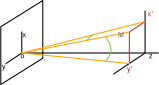
\includegraphics[scale=0.5]{approx1}
\begin{itemize}
 \item La surface S est un plan quelconque appelé plan diffractif
 \item M est proche des axes \(x',y'\)
 \item M est loin du plan diffractant
\end{itemize}
\subsubsection{Définition des angles}
On définit \(\theta_x,\theta_y\) tels que \(\sin(\theta_x)=\frac{x'}{OM}, \sin(\theta_y) = \frac{y'}{OM}\). Par les hypothèses précédentes, les angles sont très petits devant 1 et \(\sin(\theta_{x,y}) \simeq \theta_{x,y}\).
\subsubsection{Nouvelle expression de PM}
\begin{flalign*}
PM &= \sqrt{(x'-x)^2+(y'-y)^2+(z'-0)^2}\\
PM^2 &= \norm{PM}^2 \\
&= (\vec{OM}-\vec{OP})\cdot(\vec{OM}-\vec{OP})\\
&= OM^2+OP^2 - 2\vec{OM}\cdot\vec{OP} \text{ Avec } OM>>OP\\
&= OM^2(1-\frac{2\vec{OM}\cdot\vec{OP}}{OM^2}+\frac{OP^2}{OM^2}) \text{ Mais }\frac{OP}{OM}>> (\frac{OP}{OM})^2\\
PM &= OM\sqrt{1-\frac{2\vec{OM}\cdot\vec{OP}}{OM^2}}\\
&\simeq OM(1-\frac{\vec{OM}\cdot\vec{OP}}{OM^2}) \text{ Avec le DL de la racine carrée}\\
&\simeq OM - \frac{\vec{OM}}{OM}\cdot\vec{OP}\\
&\simeq OM - (x'x+y'y)/OM\\
&\simeq OM - \frac{x'x}{OM}-\frac{y'y}{OM}\\
&\simeq OM - (x\sin(\theta_x)+y\sin(\theta_y))
\end{flalign*}
Dans l'intégrale de diffraction, on a \(\frac{e^{ikPM}}{PM}\). Donc :
\begin{flalign*}
\frac{e^{ikPM}}{PM} &\simeq e^{ikOM}e^{ik(x\sin(\theta_x)+y\sin(\theta_y))}/PM\\
&\simeq e^{ikOM}e^{ik(x\sin(\theta_x)+y\sin(\theta_y))}/OM\\
\und{\psi(M)} &\simeq K\frac{e^{ikOM}}{OM}\iint\dd S \und{\psi(P)}e^{-ik(x\sin(\theta_x)+y\sin(\theta_y))}
\end{flalign*}
\begin{theorem}[Intégrale de Fraunhofer]
\[\und{\psi(M)} \simeq K\frac{e^{ikOM}}{OM}\iint\dd S \und{\psi(P)}e^{-ik(x\sin(\theta_x)+y\sin(\theta_y))}\]
\end{theorem}
\subsection{Fréquence spatiale}
On a simplifié l'intégrale en faisant appara\^itre un terme de phase linéaire en \(e^{-ik(x\sin(\theta_x)+y\sin(\theta_y))}\) associé à la fonction d'onde incidente en \(\und{\psi(P)}\).

Avec \(k = \frac{2\pi}{\lambda}\),  on peut écrire \(k\sin(\theta_x) = 2\pi \frac{\sin(\theta_x)}{\lambda} = 2\pi u\) et de m\^eme pour v. On obtient :
\begin{definition}[Fréquence spatiale au point M]
\(u = \frac{\sin(\theta_x)}{\lambda_0}\) et \(v = \frac{\sin(\theta_y)}{\lambda_0}\)
\end{definition}
On peut alors écrire la fonction comme \[\und{\psi(M)} \simeq K\frac{e^{ikOM}}{OM}\iint\dd S \und{\psi(P)}e^{-2i\pi(ux+vy)}\] qui est périodique de période \(u^{-1}\).

On obtient donc une expression ne dépendant que des angles et des fréquences spatiales. On peut le représenter en imaginant une onde diffractée subissant une homotétie au cours de la propagation.

Le motif de diffraction ne dépend que des angles introduits , donc des fréquences spatiales. On parle de direction d'observation du plan diffractant vu depuis le point M.

\subsection{Diffraction de Fraunhofer à l'infini}
Les approximations deviennent rigoureusement exactes quand on est à l'infini\marginCritical{En fait, les conditions de Fraunhofer correspondent aux conditions de Gauss dans la lentille}. On se place donc dans le plan focal image d'une lentille, ce qui nous permet d'obetnir la m\^eme chose qu'à l'infini sans la lentille.
%correspondance_le ntille schema
On a une correspondance totale entre \(M(x_i, y_i)\) et les points dans le plan focal image et on associe \(\theta_x,\theta_y\) à un point dans le pfi. On obtient alors \[\sin(\theta_x)\simeq \theta_x \simeq \frac{x_i}{f}\] On en déduit que \[u = \frac{x_i}{\lambda f_i}, v = \frac{y_i}{\lambda f_i}\]

\subsubsection{Interprétation de l'intégrale de diffraction}
C'est la somme des ondes secondaires émises depuis le point P. Il y a des intéférences avec une phase supplémantire que l'on peut interpréter géométriquement.

La différence de marche dépend uniquement de OH\marginInfo{Cela signifie que le terme \(e^{-2i\pi ux}\) montre simplement que l'onde émise en P est en avance de phase par rapport à celle émise en O} : \[\Delta \varphi = \frac{2\pi}{\lambda_0}\delta = \frac{2\pi}{\lambda_0}x\sin(\theta_x) = 2\pi ux\]
\checkInfo{Lien}{Cette partie fait le lien entre la diffraction et les interférences à l'infini.}
\section{Diffraction d'une onde plane par une fente}
\subsection{Dispositif}
\subsubsection{Onde incidente}
On prend \(\theta_{x,i}\) qui est unique et \(\theta_x\), le vecteur d'onde de l'onde incidente \(\alpha, \beta,\gamma\) est quelconque et l'onde plane s'écrit \(\psi_0 e^{-i(\omega t-\vec{k}\cdot \vec{r})}\)

On peut déterminer les composantes de k en fonction des angles : \(\alpha = \vec{k}\cdot \vec{e_x} = \norm{k}\sin(\theta_{x,i}) = 2\pi \frac{\sin(\theta_{x,i})}{\lambda_0} = 2\pi u_0\). De la m\^eme façon, on a \(\beta = 2\pi v_0\)\marginCritical{\(u_0\) est une constante alors que u dépend de x et on doit considérer toutes ses valeurs possibles.}
\subsubsection{Étude de la fente}
On considère une fente rectangulaire dans le plan Oxy centrée en O, de largeur a selon x et b selon y. L'onde reste inchangée à l'intérieur de la fente et bloquée à l'extérieur.

\subsection{Calcul de l'onde diffractée (À savoir)}
\explanation{f1}{On utilise \(\sin(\theta) = \frac{e^{i\theta}-e^{-i\theta}}{2i} \)}
\explanation{f2}{On utilise la fonction sinus cardinal. Les a et b apparaissent car dans l'expression, on divise par tout l'argument du sinus, mais a et b n'apparaissent déjà au dénominateur. Il faut donc artificiellement les introduire pour utiliser la fonction}
\begin{flalign*}
\und{\psi_(u,v)} &= K\iint \dd x \dd y \und{\psi(P)}e^{-2i\pi(ux+vy)}\\
&= K\int_{-a/2}^{a/2}\dd x\int_{-b/2}^{b/2}\dd y \psi_0 e^{-i\omega t}e^{2i\pi(u_0x+v_0y)}\times e^{-2i\pi(ux+vy)}\\
&= K\psi_0e^{-\omega t}\int_{-a/2}^{a/2}\dd x e^{-2i\pi (u-u_0)x}\int_{-b/2}^{b/2}\dd y e^{-2i\pi (v-v_0)y}\\
&= K\psi_0e^{-\omega t} [\frac{e^{-2i\pi (u-u_0)x}}{-2i\pi (u-u_0)}]_{-a/2}^{a/2} + \dots\\
&= \dots \times \frac{-1}{2i\pi (u-u_0)}(e^{-i\pi (u-u_0)a}- e^{+i\pi (u-u_0)a})\\
&= \dots \times \frac{1}{\pi (u-u_0)}\sin(\pi(u-u_0)a)\times\dots\explain{f1}{right}{0}{0.5}{×}\\
&= \dots \times a\sinc((u-u_0)a)\times\dots\explain{f2}{right}{0}{0.5}{×}\\
&= \dots \times a\sinc((u-u_0)a)b\sinc((v-v_0)b)\\
&= K' ab \times \sinc((u-u_0)a)\sinc((v-v_0)b)
\end{flalign*}
\subsection{La fonction sinus cardinal}
\warningInfo{Graphe de la fonction \(\sinc\)}{À générer sur géogébra (tracer les 2 focntions et les multiplier entre elles)}
La courbe du sinus cardinal présente un pic autour de l'origin suivi d'oscillations d'amplitude décroissantes. Elle s'annule quand \(s\neq 0\) et entier avec des extremas proche de s demi-entier.

L'effet de la multiplication par a ou b dilate ou comprime l'axe des absices d'un facteur a ou b (pour a>1, c'est comprimé, pour a<1, c'est étiré)

Le décalage par \(u_0\) translatae la courbe de ce facteur, et la fonction est centrée en \(u_0\)
\subsection{Motif de diffraction}
On sait que \(u = \frac{x_i}{\lambda f_i}, v = \frac{y_i}{\lambda f_i}\) et on peut écrire \(u_0 = \frac{x_0}{\lambda f_i}, v_0 = \frac{y_0}{\lambda f_i}\)\marginTips{\(x_{i,0}\) est le point ou l'onde incidente convergerait s'il n'y avait pas la fente, uniquement la lentille} de sorte que \[\und{\psi(x_i,y_i)} = K'' \psi_0e^{-i\omega t}ab\sinc(\frac{a(x_i-x_0)}{\lambda f_i})\sinc(\frac{b(y_i-y_0)}{\lambda f_i})\] avec \(K''\) une constante\marginInfo{Son expression est différente de K' mais cela n'a pas d'importance}

On calcule l'intensité :
\begin{flalign*}
I = \norm{K''}|\psi_0|^2(ab)^2\sinc^2(\dots)\sinc^2(\dots)\neq |\psi_0|^2
\end{flalign*}
\criticalInfo{À retenir}{Le motif de diffraction correspond au produit de 2 fonctions $\sinc$ au carré, centrée en \(x_0,y_0\) et dilatés de facteurs \(\frac{a}{\lambda f_i}, \frac{b}{\lambda f_i}\)}
On en déduit que la tache centrale a une largeur de \(2\frac{\lambda f_i}{a}\) en x et \(2\frac{\lambda f_i}{b}\) en y.
\subsubsection{Interprétation physique}
%TODO Tracer le schema avec inkscape

On observe une tache centrale d'intensité max \(I_0\) et des lobes secondaires de faible intensité.

La tache centrale est beaucoup plus brillante que les autres, donc si la largeur de la fente est assez grande, on n'observe qu'un point central brillant.
\subsection{Propriétés du motif de diffraction}
\begin{itemize}
 \item La tache de diffraction est centrée sur l'image géométrique  \(x_0,y_0\)
 \item La tache de diffraction est d'autant plus large que la fente est petite
 \item pour s'affranhir de la diffraction, il faut une onde la plus grande possible et une fente la plus largen possible. Dans certains cas, c'est la taille des éléménts optiques qui jouent le role de l fente
 \item La diffraction  se manifeste plus pour les grandes valeurs de \(\lambda\)
 \item On peut interpréter la taille de la tache centrale en fonction de l'angle \(theta_x\) orrespondant. On trouve que cette tache corrspond à un demi-angle \(\theta_x \simeq \frac{\lambda}{a}\)
 \item Plus la longueur d'onde est grande, plus la diffraction est importantes
\end{itemize}
\subsection{Résolution d'un système optique}
Une conséquence est la limite de résolution des systèmes optiques. L'image d'un point n'est plus un point mais doit etre associé à une tache de diffraction avec une certaine largeur.
 \end{document}
